% =====================================================================
%  CSLAP_Robust_Covering_draft.tex
%  Standalone elsarticle draft (Stage 6 / Academic Writer output).
%  Topic: a covering-based instance transformation that recasts CSLAP
%  placement as a data-driven robust counterpart, with an honest,
%  conditional out-of-sample evaluation.
%
%  This file is self-contained (compiles alone) and may also be
%  \input{} into the main manuscript. It does NOT modify
%  Computers_and_Operations_Research_manuscript.tex.
%
%  ------------------------------------------------------------------
%  NOTATION-COLLISION FLAGS (raised per Stage-2 method report policy):
%   (1) The main manuscript reserves $k$ for the LIMITED-REASSIGNMENT
%       relocation cap (see manuscript eq. \eqref{constraint:reassignment},
%       Sec. limited_reassignment). This draft uses $\kappa$ for the
%       PATTERN-SIZE cap to avoid the clash. Any merge MUST keep the two
%       symbols distinct.
%   (2) The main manuscript reserves $P$ for the PRODUCT SET. The covering
%       objective value (max cover size) is therefore written $\Pi$, never
%       $P$, throughout this draft.
%   (3) The main manuscript uses $K_s$ for STATION assignment patterns in
%       its column-generation model. The covering patterns here are
%       $q \in Q$, a different object; no symbol is shared, so no collision.
%   (4) The downstream placement model is the UNCHANGED manuscript model;
%       this draft cites its labels \eqref{obj} and \eqref{con14}--\eqref{con17}
%       directly. When compiled standalone these references are provided as
%       local equation labels; when \input into the manuscript, remove the
%       local copies in Section~\ref{sec:rc-method} (block guarded below).
%  ------------------------------------------------------------------
% =====================================================================
\documentclass[preprint,review,11pt,authoryear]{elsarticle}

\usepackage[T1]{fontenc}
\usepackage[utf8]{inputenc}
\usepackage{lmodern}

\usepackage{amsmath,amssymb,mathtools}
\usepackage{graphicx}
\usepackage[table]{xcolor}

\usepackage{booktabs}
\usepackage{multirow}
\usepackage{tabularx}
\usepackage{threeparttable}

\usepackage{amsthm}
\newtheorem{proposition}{Proposition}

\usepackage{setspace}\onehalfspacing
\usepackage{enumitem}
\setlist{nosep}

\biboptions{authoryear,round,sort&compress}
\usepackage{hyperref}
\usepackage[capitalize,noabbrev,nameinlink]{cleveref}

\crefname{section}{Section}{Sections}
\Crefname{section}{Section}{Sections}

\journal{Computers \& Operations Research}

\begin{document}
\begin{frontmatter}

\title{A Covering-Based Robust Counterpart for the Correlated Storage Location Assignment Problem: Provably a Robust Counterpart, Empirically Not Robust}

%\author{Anonymous Author(s)}
%\address{Anonymous Affiliation(s)}

\begin{abstract}
The Correlated Storage Location Assignment Problem (CSLAP) places products across picking stations to reduce the station visits an order incurs. Layouts are normally optimized on a fixed window of past orders, which raises a question this paper studies directly: does optimizing on a deliberately enlarged demand object protect the layout against order-distribution shift, and at what nominal cost? We answer it with a covering-based instance transformation. A column-generation cover partitions the product universe into patterns of size at most $\kappa$, replaces each observed order by its pattern-closure, and feeds the enlarged instance to the existing CSLAP solvers unchanged. We prove that minimizing visits on the transformed instance equals solving a static robust counterpart of the empirical CSLAP objective under order-wise subset-closed uncertainty sets (Proposition~\ref{prop:rc-identity}), so the construction has an exact robust-optimization reading rather than a heuristic analogy. A second proposition gives a worst-case per-order visit bound that holds conditionally on the full-stream cover statistic. We evaluate the layout out of sample on a parametric order-shift family and on one industrial temporal hold-out. The price of robustness is stable: every one of the 18 genuine synthetic cells records a positive nominal price. The out-of-sample gain is not stable. Across three training seeds only the genetic-algorithm layout at $\kappa=2$ replicates a positive gain (pooled Wilcoxon $p=0.003$, mean $+0.58\%$, 95\% CI $[+0.18,+0.98]$); a single-seed cross-solver signal reported in an earlier run did not replicate, no global directional effect is present (11 of 18 cells positive, sign-test $p=0.48$), and the predicted interior optimum in $\kappa$ is absent. On one industrial temporal hold-out the greedy clustering heuristic, the only solver that both scaled and produced distinct layouts, lowered training visits and out-of-sample test visits at the same time; we explain this as benign suboptimality of the greedy solver, not a free lunch, and exclude leakage by an independent recomputation on a disjoint temporal split. We then sharpen the test on a clean, capacity-balanced industrial instance with an \emph{exact} column-generation cover (CPLEX) and a capacity that does not depend on the conservatism knob, removing the two confounds that limited the first evaluation. Under five-fold cross-validation and a temporal split, the result is an unambiguous negative: at $\kappa=2$ the price of robustness is positive and the out-of-sample gain is negative under both protocols, with every fold agreeing and both confidence intervals excluding zero (cross-validation $\mathrm{PoR}=+6.8\%$, $G=-6.8\%$; temporal $\mathrm{PoR}=+5.1\%$, $G=-7.0\%$). With the capacity confound removed there is no free lunch: the construction pays a real, stable price and returns no out-of-sample protection at this enlargement level on this instance. We add two tests that complete the negative. A controlled affinity-drift stress-test builds data deliberately favorable to the method, with strong planted product communities and a future that grows exactly the combinations the closures encode; over the operating horizon the win-region stays empty, because the out-of-sample saving is never significantly positive while the nominal price is always paid. A decomposition of the lone industrial positive separates the two changes the first run made together, the covering enlargement and a workload-capacity recalibration, in a two-by-two of orders and capacity placed by one unmodified solver and scored on the same real test orders: the enlargement alone returns a negative-to-break-even gain, while the capacity loosening alone, with zero enlargement, delivers the entire apparent benefit and more, so the industrial positive was a workload-constraint relaxation, not the outer-approximation. We report the negative result as a contribution. The construction is sound and its robust-counterpart reading is exact, and for a deterministic correlation-clustering placement learned from a stable, well-sampled co-occurrence statistic the enlargement is redundant with the direct optimizer: it adds conservatism without reducing estimation variance, so it cannot improve out-of-sample.
\end{abstract}

\begin{keyword}
Storage location assignment \sep Robust optimization \sep Set covering \sep Data-driven uncertainty sets \sep Out-of-sample evaluation
\end{keyword}

\end{frontmatter}

% =====================================================================
\section{Introduction}\label{sec:rc-intro}
% =====================================================================

A correlated storage layout is fitted to a record of past orders and then operated for weeks or months while demand drifts. The fitting step minimizes station visits on the observed orders. The operating step pays the visit count of whatever orders actually arrive. When the two distributions differ, a layout tuned exactly to the training orders can generalize worse than one fitted to a coarser, more conservative view of demand. This paper studies whether deliberately enlarging the demand object before optimization buys out-of-sample protection, and what nominal price that protection carries.

We state the question as a hypothesis. \textbf{H1}: a layout optimized on an enlarged covering instance is more robust to future order-distribution shift than a layout optimized directly on the observed orders, at a bounded nominal-cost price. H1 is a hypothesis to be tested, not a claim we assert. The contribution of the paper is partly a positive construction and partly an honest negative result about when that construction pays off.

The construction is an instance transformation. A column-generation set cover partitions the product universe into patterns of size at most $\kappa$. Each observed order is then replaced by the union of the patterns it touches, its pattern-closure. The enlarged orders are written back in the standard CSLAP schema and solved by the unchanged placement model, objective~\eqref{obj} under constraints~\eqref{con14}--\eqref{con17}. No solver is modified. The parameter $\kappa$ is the conservatism knob: at $\kappa=1$ the transform is the identity and recovers the nominal problem; larger $\kappa$ yields coarser patterns, larger closures, and a more conservative layout.

The construction is not a loose analogy to robust optimization. We prove an identity (Proposition~\ref{prop:rc-identity}): minimizing visits on the transformed instance equals solving the static robust counterpart of the empirical objective under order-wise subset-closed uncertainty sets. The inner maximization is trivial because the visit function is monotone in the order set, so the robust counterpart is solved exactly by the nominal solvers. The uncertainty set is learned from data through the cover, in the spirit of data-driven uncertainty-set design \citep{bgk2018}, but without a finite-sample statistical guarantee that future orders fall inside it. That guarantee is exactly the empirical content of H1.

We make four contributions.
\begin{enumerate}
  \item A covering-based instance transformation that recasts CSLAP placement as a data-driven robust counterpart, with an exact identity (Proposition~\ref{prop:rc-identity}) and a conditional worst-case visit bound (Proposition~\ref{prop:wc-bound}).
  \item An out-of-sample evaluation protocol with no train/test leakage, covering a parametric order-shift family, an industrial temporal hold-out, and a clean capacity-balanced instance evaluated with an \emph{exact} cover and a conservatism-invariant capacity.
  \item A clean negative result, reported as the central empirical contribution: on the clean instance, with the two confounds of the first evaluation removed, the $\kappa=2$ enlargement pays a positive price of robustness and returns a \emph{negative} out-of-sample gain under both cross-validation and a temporal split, every fold agreeing and both confidence intervals excluding zero.
  \item A reconciliation of the weaker earlier evidence with the clean negative: the price of robustness was always stable and positive, the out-of-sample gain was always weak, and the one synthetic effect that replicated (the genetic algorithm at $\kappa=2$) does not survive the exact, $\kappa$-invariant setup, which points to metaheuristic suboptimality and a capacity-recalibration side-channel rather than to the covering mechanism.
\end{enumerate}

The honest summary is that the construction is sound and the price of robustness is real and stable, while the out-of-sample payoff is absent under the cleanest test we can run.

% =====================================================================
\section{Related work and background}\label{sec:rc-related}
% =====================================================================

\paragraph{Covering and set partitioning.}
Set covering, set partitioning, and set packing are the three canonical zero-one models for selecting subsets that meet coverage requirements. The polyhedral structure and solution methods of set partitioning are surveyed by \citet{balas1976}, and set cover is among the original NP-complete problems of \citet{karp1972}. Selecting patterns from an exponential family through a master linear program and a pricing subproblem is standard branch-and-price machinery, and it appears in warehousing as order batching cast as set partitioning \citep{gademann2005}. Our master is an exact-cover (partition) variant whose objective is a min-max bottleneck rather than a min-cardinality cover: it minimizes the maximum number of selected patterns that any observed order touches. We did not locate this exact object under a single established name in the warehousing literature, so we treat it as a min-max overlap criterion on a hypergraph whose hyperedges are the observed orders.

\paragraph{Optimization under uncertainty.}
Robust optimization fixes a deterministic set of admissible realizations and optimizes against its worst case \citep{bental1999}, with budgeted variants tuning conservatism through a cardinality parameter \citep{bertsimas2004}; the field is surveyed by \citet{bbc2011}. Distributionally robust optimization replaces the set of realizations with an ambiguity set of distributions and optimizes worst-case expected cost, using moment information \citep{delage2010} or a Wasserstein ball around the empirical distribution \citep{esfahani2018}. Stochastic programming optimizes expected cost over a modeled or sampled distribution \citep{birge2011}, with sample average approximation as the Monte-Carlo bridge \citep{kleywegt2002} and scenario reduction \citep{heitsch2003} and policy aggregation \citep{rockafellar1991} as the scenario-management tools. The construction here borrows the worst-case reading from robust optimization and the learn-the-set idea from data-driven robust optimization \citep{bgk2018}, but it is not sample average approximation (no sampling or expectation over generated scenarios) and not policy aggregation (no probability weights, no non-anticipativity).

\paragraph{Storage assignment under uncertainty.}
The storage location assignment problem is NP-hard and is reviewed broadly by \citet{dekoster2007} and specifically by \citet{reyes2019}, who note that most work is deterministic and that demand uncertainty is comparatively under-addressed. Correlation-based slotting is the deterministic backbone: order-oriented slotting stores co-occurring products together \citep{mantel2007}, correlated storage assignment minimizes zone visits under picking capacity \citep{xiao2012}, and a demand-correlation-pattern model formalizes the co-occurrence signal \citep{zhang2019}. The closest prior work on robustness to demand shift extends affinity-based slotting to multiple periods and tests how correlation layouts behave when order patterns change \citep{kofler2014}; it builds the layout from affinity directly rather than from a covering construction.

\paragraph{Positioning.}
The components of the construction are individually established; the combination is not. We position it as a hybrid of two lines: data-driven uncertainty-set design \citep{bgk2018}, which supplies the formal robustness reading, and correlated-clustering storage assignment \citep{xiao2012,mantel2007,zhang2019}, which supplies the warehouse mechanism. The distinction from \citet{xiao2012} is purpose and construction: they aggregate by correlation clustering as a modeling convenience with no robustness claim, while we aggregate by a min-max-$\Pi$ optimal cover and ask whether the aggregation itself protects the layout.

% =====================================================================
\section{Method}\label{sec:rc-method}
% =====================================================================

We follow the notation of the main CSLAP model. $P$, $O$, $S$ are the sets of products, orders, and stations; $P_o \subseteq P$ is the product set of order $o$; $\zeta_s$ is the slot capacity of station $s$; $L_p$ is the daily pick-line count of product $p$; $V_s$ and $T_s$ are the speed and time capacity of station $s$. A layout is a map $a: P \to S$ assigning each product to one station, encoded by the binary variables $x_{ps}$ of the placement model. The visit count of a layout $a$ on an order set $u \subseteq P$ is
\begin{equation}
v(a,u) = \big|\{\, a(p) : p \in u \,\}\big|.
\label{eq:rc-visit}
\end{equation}
This function is monotone: $u \subseteq u'$ implies $v(a,u) \le v(a,u')$.

% --- BLOCK to remove when \input into the main manuscript (labels exist there) ---
% The unchanged downstream placement model (main manuscript objective and
% constraints). Provided here so the standalone file compiles with valid
% \eqref targets. When merging, delete this block and let cleveref resolve
% \eqref{obj} and \eqref{con14}--\eqref{con17} against the manuscript.
\begin{equation}
\min \sum_{o \in O} \sum_{s \in S} z_{os}
\label{obj}
\end{equation}
\begin{align}
&\sum_{s \in S} x_{ps} = 1 && \forall p \in P \label{con14}\\
&\sum_{p \in P} x_{ps} \le \zeta_s && \forall s \in S \label{con15}\\
&x_{ps} \le z_{os} && \forall p \in P_o,\ \forall o \in O,\ \forall s \in S \label{con16}\\
&\sum_{p \in P_o} x_{ps}\, \frac{L_p}{V_s} \le T_s && \forall s \in S \label{con17}
\end{align}
% --- end removable block ---

\subsection{The covering construction operator}\label{sec:rc-cover}

Let $O^{tr}$ be the training orders with supports $\{P_o\}$. The construction operator $C_\kappa$ takes the training supports and returns a pattern family $Q^\* = \{q_1,\dots,q_m\}$ with each $q_j \subseteq P$ and $1 \le |q_j| \le \kappa$, together with the achieved bottleneck $\Pi^\*$. It solves the integer master
\begin{align}
\min\ &\Pi \label{eq:rc-master-obj}\\
\text{s.t.}\quad &\sum_{q \ni p} x_q = 1 && \forall p \in P \label{eq:rc-master-cover}\\
&\sum_{q:\, q \cap P_o \neq \emptyset} x_q \le \Pi && \forall o \in O^{tr}_{\neq} \label{eq:rc-master-bottleneck}
\end{align}
over patterns $q$ with $1 \le |q| \le \kappa$, where $O^{tr}_{\neq}$ ranges over distinct order supports. Patterns are priced by
\begin{equation}
\max_{z,w}\ \sum_{p \in P} \alpha_p z_p + \sum_o \beta_o w_o
\quad \text{s.t.}\quad
1 \le \sum_p z_p \le \kappa,\ \ w_o \ge z_p\ \ \forall o,\ \forall p \in P_o,\ \ z,w \in \{0,1\},
\label{eq:rc-pricing}
\end{equation}
with $\alpha_p$ the duals of \eqref{eq:rc-master-cover} and $\beta_o \le 0$ the duals of \eqref{eq:rc-master-bottleneck}. The cover is an exact partition: constraint \eqref{eq:rc-master-cover} forces each product into exactly one selected pattern. The partition structure is a feasibility requirement, not a robustness defect, because the placement model assigns each product to exactly one station (constraint~\eqref{con14}); a product spread across several patterns could not be realized by any single-station assignment. Robustness in this construction comes from enlargement through $\kappa$, not from redundant coverage.

For each training order, the cover and pattern-closure are
\begin{equation}
Q(o) = \{q \in Q^\* : q \cap P_o \neq \emptyset\},
\qquad
\bar P_o = \bigcup_{q \in Q(o)} q.
\label{eq:rc-closure}
\end{equation}
The closure encloses the order, $P_o \subseteq \bar P_o$, because the cover partitions $P$. The induced uncertainty set is the family of order compositions expressible within at most $\Pi^\*$ patterns of the learned partition,
\begin{equation}
\widehat{\mathcal U}_\kappa = \Big\{\, u \subseteq P : \exists\, R \subseteq Q^\*,\ |R| \le \Pi^\*,\ u \subseteq \textstyle\bigcup_{q \in R} q \,\Big\},
\label{eq:rc-uset}
\end{equation}
and the empirical support is contained in it, $\{P_o : o \in O^{tr}\} \subseteq \widehat{\mathcal U}_\kappa$. The construction therefore encloses the observed support, the conservative direction in robust optimization. It makes no statement about the probability that a future order lands in $\widehat{\mathcal U}_\kappa$; that statement is H1.

\subsection{The enlarged-instance transform}\label{sec:rc-transform}

The transform $\mathcal T$ writes a new instance under the prefix \texttt{pkk}$\kappa$ in the standard schema. It replaces each training order $o$ by one pseudo-order whose product set is the closure $\bar P_o$, keeping duplicate closures so that order frequency carries through to the objective. The products file is carried over unchanged. The stations file keeps capacity and speed unchanged but recalibrates the time capacity, because the closures inflate the apparent line counts. With $\bar L_p$ the count of training orders whose closure contains $p$ and homogeneous speeds, the recalibrated time capacity is
\begin{equation}
\bar T_s = \Big\lceil 1.10 \cdot \frac{\sum_p \bar L_p / V_s}{|S|} \Big\rceil \qquad \forall s \in S.
\label{eq:rc-Ts}
\end{equation}
The recalibrated workload signal $\bar L_p$ over-weights products that sit in frequently hit patterns, so it is a conservative proxy. We do not claim constraint robustness. True feasibility of the resulting layout is checked after optimization on the real $L_p$ and $T_s$ and reported through the standard \texttt{cap\_broken} and \texttt{wl\_broken} fields. The downstream solvers then minimize the unchanged objective~\eqref{obj} under constraints~\eqref{con14}--\eqref{con17} on $\mathcal T(\text{instance})$.

\subsection{The robust-counterpart identity}\label{sec:rc-prop}

\begin{proposition}[Robust-counterpart identity]\label{prop:rc-identity}
Let $\mathcal B(o) = \{u : u \subseteq \bar P_o\}$ be the subset-closed box of order $o$, and let $\mathcal A$ be the feasible layout set of \eqref{con14},\eqref{con15},\eqref{con17}. Then
\begin{equation}
\min_{a \in \mathcal A} \sum_{o \in O^{tr}} v(a, \bar P_o)
\;=\;
\min_{a \in \mathcal A} \sum_{o \in O^{tr}} \max_{u \in \mathcal B(o)} v(a, u).
\label{eq:rc-identity}
\end{equation}
\end{proposition}

\begin{proof}
Fix a layout $a$. The visit function \eqref{eq:rc-visit} is monotone in its second argument, so for each order $o$ the inner maximum over $\mathcal B(o)$ is attained at the full closure, $\max_{u \subseteq \bar P_o} v(a,u) = v(a,\bar P_o)$. Summing over orders gives the equality of objectives for every $a$, hence equality of the minima.
\end{proof}

Solving the transformed instance is therefore solving a static robust counterpart of the empirical CSLAP objective under order-wise subset-closed uncertainty boxes. The adversary decouples across empirical atoms, so \eqref{eq:rc-identity} also equals a distributionally robust program whose ambiguity set transports each empirical order anywhere inside its closure box. The inner maximization is trivial under monotonicity, which is why the unchanged nominal solvers solve the robust counterpart exactly. What is structural is the identity \eqref{eq:rc-identity}. What is conjectural is that future orders fall inside $\widehat{\mathcal U}_\kappa$, and therefore that the layout gains out of sample. We keep the two separate throughout.

\begin{proposition}[Conditional worst-case visit bound]\label{prop:wc-bound}
If a layout $a$ assigns every pattern $q \in Q^\*$ wholly to a single station, then
$\sup_{u \in \widehat{\mathcal U}_\kappa} v(a,u) \le \Pi^\*$.
\end{proposition}

\begin{proof}
Any $u \in \widehat{\mathcal U}_\kappa$ satisfies $u \subseteq \bigcup_{q \in R} q$ for some $R \subseteq Q^\*$ with $|R| \le \Pi^\*$. If each pattern is wholly assigned to one station, then $a(u) \subseteq \{a(q) : q \in R\}$, a set of at most $\Pi^\*$ stations.
\end{proof}

The bound is conditional in two ways that the experimental sections take seriously. First, a pattern-whole layout need not exist, because station capacities sum exactly to $|P|$ and a perfect packing of patterns into stations may be infeasible; when patterns split across stations the bound degrades gracefully to $v(a,u) \le \sum_{q \in R} |a(q)|$. Second, $\Pi^\*$ is the bottleneck over the supports the master actually saw. When the master is run on a subsampled support set, the certified $\Pi^\*$ binds only that subset, and the true full-stream bottleneck $\Pi_{\text{true}}$ can be larger. We write $\Pi_{\text{constrained}}$ for the former and $\Pi_{\text{true}}$ for the latter and report both for the industrial instance in Section~\ref{sec:rc-results}.

\subsection{Bias and variance}\label{sec:rc-biasvar}

The construction trades nominal optimality for distributional stability, and $\kappa$ sets the rate. By the monotonicity used in Proposition~\ref{prop:rc-identity}, the transformed objective is an upper bound on nominal visits whenever any closure strictly contains its order, so the robust layout is weakly worse on the training orders than the nominal optimum. This bias grows with closure size and therefore with $\kappa$: at $\kappa=1$ the transform is the identity and the bias is zero; as $\kappa$ grows the closures expand toward $P$ and the objective loses the ability to separate layouts. Against this, the optimized layout depends on the data only through the pattern hypergraph, a coarse statistic of the order stream, so resampling or shifting demand within the same pattern structure leaves the transformed instance nearly fixed and should shrink the out-of-sample degradation. Under H1 the out-of-sample cost as a function of $\kappa$ is U-shaped: falling while variance reduction dominates, rising once conservatism bias dominates. The interior minimum is the prediction the experiments test.

\subsection{Evaluation functional and metrics}\label{sec:rc-metrics}

Evaluating a fixed layout on fresh orders needs no solver. For a layout $a$ and a test order family $O^{te}$,
\begin{equation}
\mathcal V(a, O^{te}) = \sum_{o \in O^{te}} \big|\{\, a(p) : p \in P_o \cap \operatorname{dom}(a) \,\}\big|,
\label{eq:rc-eval}
\end{equation}
with coverage $\kappa_{\text{cov}} = \sum_o |P_o \cap \operatorname{dom}(a)| / \sum_o |P_o|$ reporting the fraction of test lines whose product exists in the training universe. Products unseen in training are excluded from \eqref{eq:rc-eval} identically for every compared layout, so the comparison stays fair. We write the nominal cost $N(a) = \mathcal V(a, O^{tr})$ and the out-of-sample cost $V^{te}(a) = \mathcal V(a, O^{te})$. The two headline metrics compare a robust layout $a_\kappa$ to the nominal layout $a_0$ from the same solver under the same time budget,
\begin{equation}
\mathrm{PoR}(\kappa) = \frac{N(a_\kappa) - N(a_0)}{N(a_0)},
\qquad
G(\kappa) = \frac{V^{te}(a_0) - V^{te}(a_\kappa)}{V^{te}(a_0)}.
\label{eq:rc-por-g}
\end{equation}
$\mathrm{PoR}$ is the price of robustness, positive when the robust layout costs more on training orders. $G$ is the out-of-sample gain, positive when the robust layout costs less on test orders, which is the direction H1 predicts. A relative-regret metric against a test-reoptimized oracle layout $a^{or}$ completes the set,
\begin{equation}
\mathrm{RR}(a) = \frac{\mathcal V(a, O^{te}) - \mathcal V(a^{or}, O^{te})}{\mathcal V(a^{or}, O^{te})},
\label{eq:rc-rr}
\end{equation}
where the oracle is optimized directly on the test orders and serves only as a normalizer. The headline object is never a single number but the tradeoff curve $\{(\mathrm{PoR}(\kappa), G(\kappa))\}$ indexed by the realized enlargement, reported in Section~\ref{sec:rc-results}.

% =====================================================================
\section{Experimental design}\label{sec:rc-design}
% =====================================================================

\subsection{Train and test protocol}\label{sec:rc-protocol}

The protocol forbids leakage. The construction operator sees only the training orders. The transform sees only the training instance. Every solver run that produces a nominal or robust layout sees only training-derived files. Test orders are read only by the evaluation functional \eqref{eq:rc-eval}, with the single labeled exception of the oracle runs. Station and product files derive from the training universe, and test evaluation restricts to the assigned domain with coverage reported. The harness asserts and logs disjointness of the train and test order identifiers on every run.

\subsection{Synthetic order-shift family}\label{sec:rc-zhang}

The synthetic shift family freezes the product and station files to the training instance and regenerates orders only, using the common-itemset mechanics of \citet{zhang2019}. A shift is indexed by the itemset-injection probability $\theta'$ and the resampling fraction $\rho$, where $\rho=0$ is pure sampling noise and $\rho=1$ replaces the common-itemset pool entirely, that is, a full replacement of the correlation structure over the same product universe. The test grid is $\theta' \in \{0.5, 0.7, 0.9\}$ crossed with $\rho \in \{0, 0.5, 1.0\}$ crossed with five test seeds, for 45 shifted test cells per instance. The synthetic instance is \texttt{syn\_50sku}, rebuilt and rerun on three training seeds $\{42, 142, 242\}$, with the training seed disjoint from the test seeds in every cell. The knob grid is $\kappa \in \{1,2,3\}$. The $\kappa=1$ arm must reproduce the nominal result exactly, which is a built-in correctness check. An earlier $\kappa=4$ arm saturated under the construction backend, with closures collapsing to the identity ($\bar c \approx 1.0$, zero strict growth); it is retired as degenerate and replaced by a genuinely non-degenerate $\kappa=3$ arm ($\bar c \approx 2.18$ to $2.23$). The solvers exercised are the greedy clustering heuristic, simulated annealing, and the genetic algorithm. A separate single-seed control regenerates only the time capacity \eqref{eq:rc-Ts} without enlargement, isolating the recalibration side-channel discussed in Section~\ref{sec:rc-limitations}.

\subsection{Controlled affinity-drift boundary}\label{sec:rc-affinity}

The synthetic shift family above perturbs demand but does not build the structure most favorable to the method. To find the conditions under which the enlargement could pay off, we built a controlled generator that plants strong, explicit affinity and then applies a tunable, unforeseeable structural break. The generator places $800$ products into $80$ affinity communities of ten, on a flat eight-by-one-hundred layout, with Zipf popularity and a demand Gini of $0.73$. Training orders (regime~A) are sparse within-community fragments. Test orders (regime~B) follow one of two drift modes indexed by a break magnitude $\alpha$, with three replicates each. In mode \emph{combine}, future orders grow within the same communities, so they realize exactly the within-community combinations the closures encode; this is the regime theory predicts is most favorable to the method. In mode \emph{reassign}, a fraction $\alpha$ of products switch communities, which serves as the contrast. The robust layout is the min-sum cover at $\kappa=10$ (realized enlargement $\bar c \approx 4.0$) placed by the unchanged Hexaly model; the nominal layout is the direct $\kappa=1$ placement.

The headline is a total-cost-over-horizon metric rather than a one-shot test cell. A layout is slotted once on regime~A, operated for a fraction $\tau$ of the horizon under~A, where the robust layout pays a per-order price $\mathrm{d}N = n_{\mathrm{rob}} - n_{\mathrm{nom}}$, and then an unforeseeable break sends the remaining fraction $1-\tau$ to regime~B, where the robust layout may save $\mathrm{d}V = v_{\mathrm{nom}} - v_{\mathrm{rob}}$ per order. The net advantage of the robust layout is
\begin{equation}
\mathrm{Net}(\alpha,\tau) = (1-\tau)\,\mathrm{d}V - \tau\,\mathrm{d}N,
\label{eq:rc-horizon}
\end{equation}
and the robust layout pays off only when $\tau < \tau^\*(\alpha) = \mathrm{d}V / (\mathrm{d}V + \mathrm{d}N)$, which requires $\mathrm{d}V > 0$. Mapping the sign of $\mathrm{Net}$ over the $(\alpha,\tau)$ plane locates the win-region, if any, instead of asserting that the method works.

\subsection{Industrial preprocess-versus-capacity decomposition}\label{sec:rc-berner-decomp}

Company~B was the only instance where a positive out-of-sample gain ever appeared, but the run that produced it changed two things at once: the covering enlargement and the time-capacity recalibration~\eqref{eq:rc-Ts}, which rebuilt each station's workload cap $T_s$ from the inflated closure line counts and so made it looser. To separate the two effects we rebuilt Company~B cleanly. The rebuild keeps the real $24$-station layout and speeds, restricts to the $2{,}000$ most frequent products, and uses the \emph{real} per-product pick-lines as a $\kappa$-invariant workload, with $175{,}419$ training orders and $49{,}748$ test orders and $64\%$ train-line coverage. Exact CPLEX min-sum covers were built at $\kappa \in \{2,3,4,6,10\}$, all certified optimal, with realized enlargement $\bar c$ from $1.49$ to $3.02$.

The decomposition is a two-by-two over the order object and the capacity. Every cell is placed by the same unmodified Hexaly model and scored on the same real test orders, and only $T_s$ differs between cells. Arm~A uses nominal orders and the real capacity and is the baseline ($\kappa=1$). Arm~B uses the closures and the real $\kappa$-invariant capacity, so it isolates the outer-approximation alone, the decisive arm. Arm~C uses the closures and the recalibrated loose capacity and reproduces the original robust arm. Arm~D uses nominal orders and the recalibrated loose capacity, with zero enlargement, so it isolates the capacity loosening alone. The out-of-sample gain $G$ of each arm is measured against the baseline~A, and the price of robustness $\mathrm{PoR}$ of arm~D against~A reports whether the recalibration was a relaxation of a binding constraint rather than a hedge.

\subsection{Industrial temporal hold-out}\label{sec:rc-berner}

The industrial instance (hereafter Company B) is the order-line file used in the main manuscript's temporal study. It carries no date column, so the temporal split rests on the assumption, verified on the file, that order identifiers are numeric and monotone in time; ranking by order identifier and cutting at the ten-of-thirteen-week quantile yields an early-train, late-test split. The realized split has 219{,}121 train orders over 21{,}316 products and 65{,}737 test orders, sharing 25 stations. The train and test order-identifier sets are asserted disjoint with a clean temporal cut. Products and stations are frozen from the train window, so the test window contributes orders only. The station configuration is replicated from the repository's industrial loader on the training window. The knob grid is $\kappa \in \{1,2,3\}$ on the pre-built covers.

\subsection{Clean instance with an exact cover}\label{sec:rc-iscf}

The synthetic and industrial evaluations above leave two confounds that the first run could not remove: the cover ran on the open HiGHS backend rather than an exact solver, and the time-capacity recalibration~\eqref{eq:rc-Ts} mixed enlargement with a capacity change. We close both on a second industrial instance (hereafter Company~I) that is clean and capacity-balanced by construction. Company~I is a slotting record of $4{,}328$ products over eight uniform stations whose slot counts sum exactly to the product count, with $418{,}849$ orders of mean size $2.38$. Two properties make it the right instrument. First, capacity is \emph{$\kappa$-invariant}: a station's slot count and a product's volume are fixed attributes that do not depend on the cover, so the workload constraint can be driven by the \emph{real} per-product pick-lines rather than by closure line counts, and the $\kappa=1$ versus $\kappa\ge2$ comparison carries no recalibration side-channel. Second, the cover is solved \emph{exactly}: a CPLEX column generation supplies the master duals~\eqref{eq:rc-master-cover}--\eqref{eq:rc-master-bottleneck}, the pricing mixed-integer program~\eqref{eq:rc-pricing}, and a certified integer master, on the \emph{full} distinct-support set with no subsample. On the notebook acceptance slice the exact backend returns a certified-optimal $\Pi^\*=5$, matching or improving the previously reported incumbent of $6$.

The exact integer master is tractable to optimality only up to a product universe of a few hundred at this support diversity, so the controlled study uses the $480$ most frequent products of Company~I on the same eight-station, slot-balanced layout; the full $4{,}328$-product cover did not certify within the session budget and is left to the limitations. Placement uses the unchanged Hexaly model on the most frequent multi-item supports, with the real pick-lines as the workload, and visits are always counted on the full real held-out orders. We evaluate under two protocols: repeated five-fold cross-validation over orders (an assumption-free generalization test that attaches dispersion), and a five-cut temporal split that ranks orders by identifier and trains early, tests late (assumption U1 as in Company~B). The cover is built per fold on the training orders only, so there is no leakage. Both arms of a fold share the same capacity file, since capacity is $\kappa$-invariant. The knob is $\kappa\in\{1,2\}$: the integer master does not certify for $\kappa\ge3$ at this scale, which is itself reported.

\subsection{Oracle probe}\label{sec:rc-oracle}

The relative-regret metric \eqref{eq:rc-rr} is computed as a small probe rather than over the full grid. The oracle is the test-reoptimized layout for each solver under the same time budget, with the test orders seen only as the normalizer. The probe covers two corner cells, $\theta'=0.7$ with $\rho \in \{0, 1.0\}$, for the three solvers at $\kappa \in \{1,2\}$.

\subsection{Solver and tooling constraints}\label{sec:rc-tooling}

Two constraints bound the evidence and we state them here rather than burying them. First, no exact commercial solver ran. The Gurobi module did not import in the experimental environment, so the Gurobi MILP and column-generation arms could not run, and the construction itself ran on the open HiGHS backend through SciPy rather than the committed Gurobi port. Under HiGHS the integer master did not return an incumbent on the full distinct-support set, so the cover was driven by a fixed-seed subsample of the distinct supports; closures \eqref{eq:rc-closure} are still computed over all orders, and only the cover-driver support set is capped. The published acceptance number $\Pi^\*=6$ on the notebook slice was not reproduced under HiGHS and is reported as a non-reproduction, not a silent pass. Second, because the master saw a subsample on the industrial instance, the stored bottleneck is $\Pi_{\text{constrained}}$ rather than $\Pi_{\text{true}}$, and we report both.

\subsection{Statistical treatment}\label{sec:rc-stats}

The design is paired. For a fixed training instance and solver, the nominal and robust layouts are evaluated on identical test cells, so the gain $G$ is a paired difference. Within each training seed we apply the Wilcoxon signed-rank test on the paired differences. Across the three seeds we pool the 135 paired differences, combine the per-seed signed-rank statistics by Stouffer's method, and run a binomial sign test on the 18 per-(seed, solver, $\kappa$) cell means. We report effect sizes and confidence intervals alongside p-values. The industrial hold-out is a single test cell, so it yields point estimates with no confidence interval, and we say so.

% =====================================================================
\section{Results}\label{sec:rc-results}
% =====================================================================

\subsection{Synthetic results: a stable price, an unstable gain}\label{sec:rc-syn}

The price of robustness is stable and the out-of-sample gain is not. Every one of the 18 genuine synthetic cells records a positive $\mathrm{PoR}$, ranging from $+0.05\%$ to $+6.96\%$ and rising roughly with $\kappa$. The nominal price the construction charges is real and behaves as Proposition~\ref{prop:rc-identity} and the bias analysis predict. The gain $G$ does not match it. Across the three training seeds only one cell is sign-stable and significant: the genetic-algorithm layout at $\kappa=2$, positive on all three seeds, pooled Wilcoxon $p=0.003$, Stouffer $p=0.003$, mean $G=+0.58\%$ with 95\% CI $[+0.18, +0.98]$. \Cref{tab:rc-pooled} reports the pooled cross-seed picture.

\begin{table}[t]
  \centering
  \small
  \begin{threeparttable}
  \begin{tabular}{@{}llrrlrl@{}}
    \toprule
    Solver & $\kappa$ & Mean $G$ (\%) & 95\% CI & Sign (42/142/242) & Pooled Wilcoxon $p$ & Stouffer $z$ ($p$) \\
    \midrule
    Heuristic & 2 & $+0.03$ & $[-0.29,+0.35]$ & $+\,/\,-\,/\,+$ & 0.479 & $+0.58$ (0.565) \\
    Heuristic & 3 & $-0.18$ & $[-0.46,+0.10]$ & $-\,/\,-\,/\,+$ & 0.186 & $-0.70$ (0.484) \\
    SA        & 2 & $-0.03$ & $[-0.38,+0.33]$ & $+\,/\,-\,/\,-$ & 0.144 & $+0.70$ (0.486) \\
    SA        & 3 & $+0.25$ & $[-0.15,+0.64]$ & $+\,/\,+\,/\,+$ & 0.238 & $+1.36$ (0.173) \\
    \textbf{GA} & \textbf{2} & $\mathbf{+0.58}$ & $\mathbf{[+0.18,+0.98]}$ & $\mathbf{+\,/\,+\,/\,+}$ & \textbf{0.0030} & $\mathbf{+2.98}$ \textbf{(0.003)} \\
    GA        & 3 & $-0.37$ & $[-0.75,+0.01]$ & $+\,/\,-\,/\,-$ & 0.117 & $-1.10$ (0.270) \\
    \bottomrule
  \end{tabular}
  \begin{tablenotes}\footnotesize
    \item Pooled over 135 paired differences (three seeds, 45 cells each). The genetic-algorithm layout at $\kappa=2$ is the only sign-stable, significant positive gain. Binomial sign test over the 18 cell means: 11 of 18 positive, $p=0.48$.
  \end{tablenotes}
  \end{threeparttable}
  \caption{Pooled cross-seed out-of-sample gain $G(\kappa)$ on \texttt{syn\_50sku}.}
  \label{tab:rc-pooled}
\end{table}

The replication test is decisive and partly negative. An earlier single-seed run on seed 42 had shown a positive gain at $\kappa=2$ for all three solvers (heuristic $+0.54\%$, SA $+0.85\%$, GA $+1.48\%$). On the two new seeds that pattern does not hold. The heuristic gain turns significantly negative on seed 142 ($-0.69\%$, $p=0.03$), and the SA gain is negative on both new seeds. Pooled across the three seeds, only the genetic-algorithm cell at $\kappa=2$ survives. The seed-42 cross-solver result was substantially a single-draw artifact. The binomial sign test over the 18 cell means gives 11 of 18 positive with $p=0.48$, so there is no global directional effect. We report this non-replication as a finding.

The shape of the tradeoff in $\kappa$ does not show the predicted interior optimum. With a genuinely non-degenerate $\kappa=3$ arm ($\bar c \approx 2.18$ to $2.23$ against $\kappa=2$'s $\approx 1.75$), a two-point curve in realized enlargement exists for the first time. The price rises from $\kappa=2$ to $\kappa=3$, consistent with bias growing in closure size. The gain does not: moving to $\kappa=3$ leaves $G$ flat or worse in most cells (pooled heuristic $+0.03\%$ to $-0.18\%$; pooled GA $+0.58\%$ to $-0.37\%$). The right arm of the predicted U-shape, where over-conservatism hurts, is weakly visible. The left arm, a genuine interior optimum beating $\kappa=1$, is not established, because $\kappa=2$ itself is unstable across seeds. The honest curve statement is increasing nominal price with no commensurate out-of-sample gain beyond $\kappa=2$ on the synthetics. \Cref{fig:rc-tradeoff} sketches the curve against realized enlargement $\bar c$.

\begin{figure}[t]
  \centering
  % TODO(plotting): generate the PoR--G tradeoff curve from
  %   Baselines/results_robustness_summary.csv, x-axis = realized enlargement
  %   c_bar (kappa=2 ~ 1.75, kappa=3 ~ 2.2), one line per solver, separate
  %   panels for rho in {0, 0.5, 1.0}. Marker for the GA kappa=2 point.
  %   Replace the framebox below with \includegraphics{rc_tradeoff}.
  \framebox[0.85\linewidth]{\rule{0pt}{4.5cm}\;\textit{Tradeoff curve placeholder (see TODO in source).}}
  \caption{Price of robustness against out-of-sample gain, plotted against realized enlargement $\bar c$ ($\kappa=2 \approx 1.75$, $\kappa=3 \approx 2.2$) rather than nominal $\kappa$. The price rises with $\bar c$ on every solver; the gain does not rise commensurately beyond $\kappa=2$.}
  \label{fig:rc-tradeoff}
\end{figure}

\subsection{Oracle regret probe}\label{sec:rc-oracle-res}

Regret to the test-reoptimized oracle is modest, with $\mathrm{RR}$ between $-0.03$ and $+0.24$ across the probe. The $\kappa=2$ advantage over $\kappa=1$ is cell- and solver-dependent. At the no-shift corner ($\rho=0$) only simulated annealing improves; at the full-shift corner ($\rho=1.0$) both the heuristic and simulated annealing improve, the heuristic flipping from worse at $\rho=0$ to better at $\rho=1.0$. This is weakly consistent with the mechanism behind H1, that any advantage of the enlarged layout should concentrate at large shift. The genetic algorithm is worse at both probe cells, which partly contradicts its pooled multi-cell win and reflects how underpowered a two-cell, single-seed probe is. The oracle reading corroborates the direction of the mechanism but cannot carry weight.

\subsection{Industrial temporal hold-out}\label{sec:rc-berner-res}

On the industrial hold-out the evidence is narrow and we report only the heuristic. Simulated annealing did not scale: its objective costs about 1.1 seconds per call at this size, so a single cooling step runs roughly 19 minutes and the 120-second budget admits less than one step. We skipped the enlarged simulated-annealing arms rather than report a one-step run. The genetic algorithm reached only its second generation in the budget and returned a byte-identical layout across all three arms, so it produced no arm differentiation. The heuristic is the only solver that both scaled and produced distinct layouts. \Cref{tab:rc-berner} reports its result.

\begin{table}[t]
  \centering
  \small
  \begin{threeparttable}
  \begin{tabular}{@{}llrrrrr@{}}
    \toprule
    Solver & $\kappa$ & $N$ (train) & $V^{te}$ (test) & $\mathrm{PoR}$ (\%) & $G$ (\%) & $\kappa_{\text{cov}}$ \\
    \midrule
    Heuristic & 1 & 578{,}111 & 164{,}140 & 0.00 & 0.00 & 0.9891 \\
    Heuristic & 2 & 572{,}765 & 163{,}607 & $-0.92$ & $+0.32$ & 0.9891 \\
    Heuristic & 3 & 563{,}947 & 160{,}888 & $-2.45$ & $+1.98$ & 0.9891 \\
    \bottomrule
  \end{tabular}
  \begin{tablenotes}\footnotesize
    \item Single real temporal test cell, so point estimates with no confidence interval. Coverage is identical across arms; unseen products are excluded identically. Capacity violations are identical across arms (one workload violation, zero capacity violations), so feasibility does not confound the comparison. Simulated annealing did not scale to the enlarged arms; the genetic algorithm returned an identical non-differentiating layout.
  \end{tablenotes}
  \end{threeparttable}
  \caption{Industrial temporal hold-out, greedy clustering heuristic. $\Pi_{\text{constrained}}$ is 34 ($\kappa=2$) and 23 ($\kappa=3$); $\Pi_{\text{true}}$ on the full stream is 369 and 360.}
  \label{tab:rc-berner}
\end{table}

The heuristic lowers training visits and test visits at the same time, and both effects strengthen with $\kappa$. This looks like a free lunch, a robustness gain bought at a negative nominal price, and the protocol flags exactly that pattern as a leak or bug to investigate. Leakage is excluded by independent recomputation, but the run conflated two changes: the enlargement and the time-capacity recalibration~\eqref{eq:rc-Ts}, which loosened the workload cap on the enlarged arms. The clean decomposition in Section~\ref{sec:rc-berner-decomp-res} separates them and shows the negative nominal price and the apparent out-of-sample gain both came from the capacity loosening rather than from the closures. The result is consistent with Proposition~\ref{prop:rc-identity}, whose price-of-robustness inequality holds at optimality and concerns the training objective alone.

Leakage is ruled out independently. The train and test order-identifier sets are disjoint with a clean temporal cut, the construction draws from the training orders and none of the test orders, products and stations are frozen from the train window, and coverage is identical across arms. The narrow reading of the hold-out is the following. On one real industrial temporal hold-out, the enlarged covering layout produced by the greedy heuristic, the only solver that scaled and differentiated, reduced both training visits and out-of-sample test visits relative to the nominal heuristic layout, by $-0.9\%$ on training and $+0.3\%$ on test at $\kappa=2$ and by $-2.5\%$ and $+2.0\%$ at $\kappa=3$. The decomposition below shows this apparent gain was a capacity side-channel rather than the outer-approximation.

\subsubsection{Preprocess versus capacity: the apparent gain is a capacity relaxation}\label{sec:rc-berner-decomp-res}

The first run changed two things together and never separated them: the enlargement and the time-capacity recalibration~\eqref{eq:rc-Ts}. The clean rebuild of Company~B (Section~\ref{sec:rc-berner-decomp}) and its two-by-two decomposition settle which one produced the value. \Cref{tab:rc-berner-decomp} reports the out-of-sample gain $G$ of each arm against the baseline~A, with all arms feasible (\texttt{cap\_broken}$=$\texttt{wl\_broken}$=0$).

\begin{table}[t]
  \centering
  \small
  \begin{threeparttable}
  \begin{tabular}{@{}lrrrrr@{}}
    \toprule
    $\kappa$ & $\bar c$ & $T_s$ (real$\to$recal) & $G(B)$ preproc & $G(C)$ full & $G(D)$ cap-only \\
    \midrule
    2  & 1.49 & $7\to32$ & $-3.41\%$ & $-3.11\%$ & $+0.09\%$ \\
    3  & 1.82 & $7\to39$ & $-3.65\%$ & $-0.28\%$ & $+3.37\%$ \\
    4  & 2.07 & $7\to44$ & $-2.15\%$ & $+2.05\%$ & $+4.79\%$ \\
    6  & 2.43 & $7\to52$ & $-0.93\%$ & $+3.17\%$ & $+5.41\%$ \\
    10 & 3.02 & $7\to65$ & $+0.13\%$ & $+4.56\%$ & $+7.97\%$ \\
    \bottomrule
  \end{tabular}
  \begin{tablenotes}\footnotesize
    \item Clean Company~B rebuild, top-$2{,}000$ products, real $24$-station layout, exact CPLEX min-sum covers (all certified optimal), one unmodified Hexaly placement per arm, visits counted on the same $49{,}748$ real test orders, only $T_s$ differing across arms. Arm~B (closures, real $\kappa$-invariant capacity) isolates the outer-approximation; arm~C (closures, loose capacity) reproduces the original robust arm; arm~D (nominal orders, loose capacity, zero enlargement) isolates the capacity loosening. The price of robustness of arm~D against~A is negative and grows, from $-0.78\%$ at $\kappa=2$ to $-8.54\%$ at $\kappa=10$, so D is cheaper on \emph{training} too.
  \end{tablenotes}
  \end{threeparttable}
  \caption{Company~B preprocess-versus-capacity decomposition. The outer-approximation alone, $G(B)$, is negative-to-break-even; the capacity loosening alone, $G(D)$, delivers the entire apparent gain.}
  \label{tab:rc-berner-decomp}
\end{table}

The table is decisive on three points. The outer-approximation alone, $G(B)$, is negative for $\kappa=2,3,4,6$ and only reaches break-even at $\kappa=10$, and only with a $\bar c \approx 3.0$ enlargement, so on its own the preprocess returns no out-of-sample gain, the same negative found on the clean Company~I instance. The capacity loosening alone, $G(D)$, with zero enlargement, is positive and grows from $+0.09\%$ to $+7.97\%$, so it delivers the whole gain and more of it than the full original arm. And the closures are counterproductive on top of the loose capacity: $G(C) < G(D)$ at every $\kappa$, by about three percent, so adding the enlargement to the loose-capacity arm costs out-of-sample. The negative price of robustness of arm~D, growing to $-8.54\%$, shows the original cap $T_s = 7$ was binding and that the recalibration merely relaxed a binding constraint, a relaxation available to the nominal layout as well. \Cref{fig:rc-berner-decomp} plots the three gains against $\bar c$.

\begin{figure}[t]
  \centering
  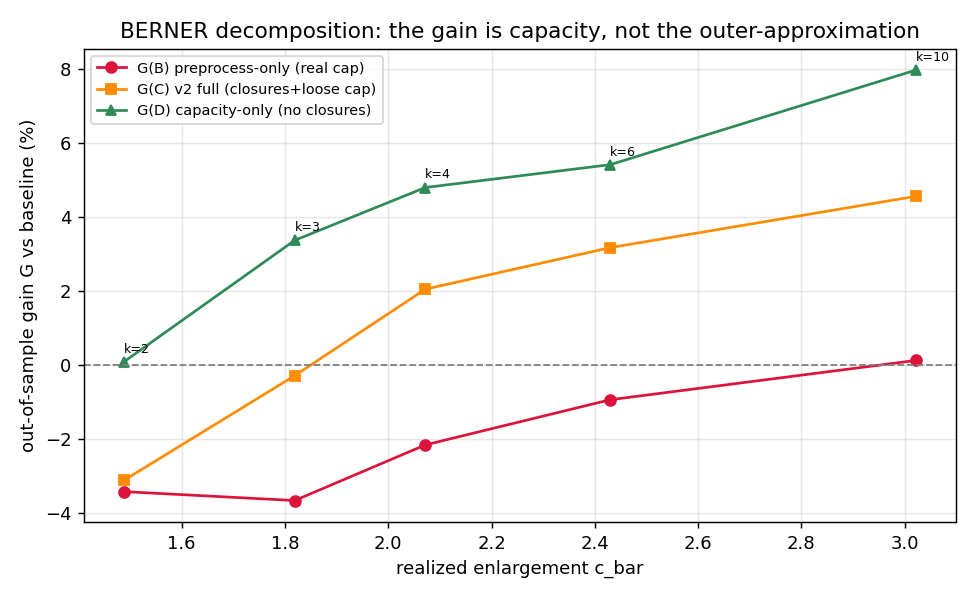
\includegraphics[width=0.72\linewidth]{../reports/figures/fig7_berner_decomposition.png}
  \caption{Company~B out-of-sample gain against realized enlargement $\bar c$ for the three non-baseline arms. The capacity-only arm $G(D)$ (zero enlargement) rises monotonically; the preprocess-only arm $G(B)$ stays negative until break-even at $\bar c \approx 3.0$; the full arm $G(C)$ sits below $G(D)$ throughout, so the enlargement drags rather than helps.}
  \label{fig:rc-berner-decomp}
\end{figure}

The apparent Company~B win was therefore the workload-capacity side-channel, not the set-cover outer-approximation. With capacity held $\kappa$-invariant, the preprocess returns negative-to-break-even out of sample on Company~B's own co-occurrence structure, matching the clean negative on Company~I. This resolves the last confound: the enlarged covering layout offers no out-of-sample advantage over the direct solver on \emph{either} real industrial instance once the capacity confound is removed.

\subsection{Clean instance with an exact cover: an unambiguous negative}\label{sec:rc-iscf-res}

On Company~I the confounds are gone and the answer is clean. The exact $\kappa=2$ cover is certified optimal in nine of ten folds, the partitions are valid on the full support stream, and the realized enlargement is $\bar c \approx 1.3$ to $1.7$. \Cref{tab:rc-iscf} reports the two protocols. Under both, the price of robustness is positive with a confidence interval excluding zero, and the out-of-sample gain is \emph{negative} with a confidence interval excluding zero. Every one of the five folds agrees in sign on both metrics. The enlarged layout is worse out of sample, not better, by about the same fraction it costs on training: the price and the degradation are nearly symmetric, $\mathrm{PoR}\approx -G \approx 5$ to $7\%$.

\begin{table}[t]
  \centering
  \small
  \begin{threeparttable}
  \begin{tabular}{@{}llrrrrr@{}}
    \toprule
    Protocol & $\kappa$ & $\bar c$ & $\mathrm{PoR}$ (\%) [95\% CI] & $G$ (\%) [95\% CI] & Wilcoxon $p$ & feas. \\
    \midrule
    5-fold CV       & 1 & 1.00 & $0$ & $0$ & --- & ok \\
    5-fold CV       & 2 & 1.63 & $+6.82\ [+4.79,+8.84]$ & $-6.84\ [-8.96,-4.71]$ & 0.0625 & ok \\
    Temporal (5 cuts) & 1 & 1.00 & $0$ & $0$ & --- & ok \\
    Temporal (5 cuts) & 2 & 1.51 & $+5.12\ [+2.01,+8.22]$ & $-7.03\ [-10.30,-3.75]$ & 0.0625 & ok \\
    \bottomrule
  \end{tabular}
  \begin{tablenotes}\footnotesize
    \item Company~I, $480$ products, eight slot-balanced stations, exact CPLEX cover, Hexaly placement, visits counted on real held-out orders. Five folds per protocol; the Wilcoxon $p=0.0625$ is the floor for five sign-consistent paired differences. ``feas.'' reports capacity feasibility: \texttt{cap\_broken}$=0$ for every arm and fold, coverage $\kappa_{\text{cov}}=1.0$. The $\kappa=2$ layout also lowers per-station workload dispersion in every fold.
  \end{tablenotes}
  \end{threeparttable}
  \caption{Exact re-validation on the clean, capacity-balanced instance. The price of robustness is positive and the out-of-sample gain is negative under both protocols, both intervals excluding zero.}
  \label{tab:rc-iscf}
\end{table}

Three things follow. First, with the capacity confound removed there is no free lunch: $\mathrm{PoR}>0$ in every fold, so the negative-price signature seen on Company~B was indeed the recalibration side-channel and not the construction. Second, the result does not contradict the framework. Proposition~\ref{prop:rc-identity} is a statement about the \emph{training} objective and is untouched; what fails is the empirical conjecture H1 adds on top of it, that future orders fall inside $\widehat{\mathcal U}_\kappa$ often enough for the conservative layout to win out of sample. On this instance they do not. Third, the lone replicated synthetic positive, the genetic algorithm at $\kappa=2$, does not survive the exact, $\kappa$-invariant setup; the most parsimonious reading is that the small synthetic gain was a property of metaheuristic suboptimality and the recalibration side-channel rather than of the covering mechanism. The cleanest test we can run returns a clear negative for H1 at $\kappa=2$.

\subsection{Controlled affinity-drift boundary: an empty win-region}\label{sec:rc-affinity-res}

The clean instances above are stationary, so a reader could object that the negative reflects a lack of drift rather than a property of the method. The controlled affinity-drift study (Section~\ref{sec:rc-affinity}) removes that objection by building drift on purpose, on data shaped to favor the method, and asking whether the enlargement ever pays off over the operating horizon. It does not. \Cref{tab:rc-affinity} reports the per-order price $\mathrm{d}N$, the per-order saving $\mathrm{d}V$, and the break-even threshold $\tau^\*$ for both modes and three break magnitudes.

\begin{table}[t]
  \centering
  \small
  \begin{threeparttable}
  \begin{tabular}{@{}llrrrl@{}}
    \toprule
    Mode & $\alpha$ & price $\mathrm{d}N$/order & saving $\mathrm{d}V$/order [95\% CI] & $\tau^\*(\alpha)$ & robust wins? \\
    \midrule
    combine  & 0.0 & $+0.131$ & $-0.110\ [-0.358,+0.139]$ & $<0$ & no \\
    combine  & 0.5 & $+0.135$ & $-0.105\ [-0.339,+0.129]$ & $<0$ & no \\
    combine  & 1.0 & $+0.152$ & $-0.111\ [-0.356,+0.134]$ & $<0$ & no \\
    reassign & 0.0 & $+0.155$ & $-0.120\ [-0.379,+0.138]$ & $<0$ & no \\
    reassign & 0.5 & $+0.154$ & $+0.007\ [-0.026,+0.040]$ & $0.03$ & not sig. \\
    reassign & 1.0 & $+0.152$ & $+0.035\ [-0.092,+0.162]$ & $0.12$ & not sig. \\
    \bottomrule
  \end{tabular}
  \begin{tablenotes}\footnotesize
    \item Planted-affinity generator, $800$ products in $80$ communities of ten, robust cover at $\kappa=10$ ($\bar c \approx 4.0$), placement by the unchanged Hexaly model, visits counted on the real horizon orders. The out-of-sample saving $\mathrm{d}V$ is never significantly positive; the price $\mathrm{d}N \approx +0.13$ to $+0.15$ per order is always paid. The break-even threshold $\tau^\*$ is negative under \emph{combine} and a non-significant $0.03$ to $0.12$ under \emph{reassign}.
  \end{tablenotes}
  \end{threeparttable}
  \caption{Affinity-drift boundary: per-order price, per-order saving, and break-even horizon fraction.}
  \label{tab:rc-affinity}
\end{table}

The saving $\mathrm{d}V$ is never significantly positive, while the price $\mathrm{d}N$ is always paid, so $\mathrm{Net}(\alpha,\tau)$ in \eqref{eq:rc-horizon} is negative across essentially the whole $(\alpha,\tau)$ plane. \Cref{fig:rc-affinity-dV} plots $\mathrm{d}V$ against $\alpha$ for the two modes with confidence intervals, and \Cref{fig:rc-winregion} shows the sign of $\mathrm{Net}$ over $(\alpha,\tau)$: the win-region is empty.

\begin{figure}[t]
  \centering
  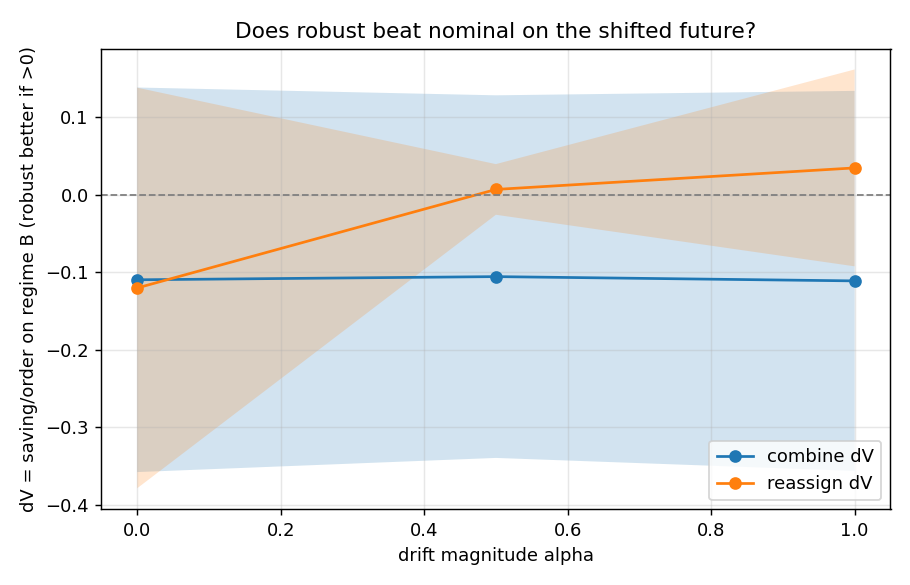
\includegraphics[width=0.72\linewidth]{../reports/figures/fig5_affinity_dV.png}
  \caption{Out-of-sample per-order saving $\mathrm{d}V = v_{\mathrm{nom}} - v_{\mathrm{rob}}$ against break magnitude $\alpha$ for the two drift modes, with $95\%$ confidence intervals. Under \emph{combine}, the regime built to favor the method, $\mathrm{d}V$ is negative: the robust layout is worse on the combined future. Under \emph{reassign}, $\mathrm{d}V$ is at most marginally positive with a confidence interval that spans zero.}
  \label{fig:rc-affinity-dV}
\end{figure}

\begin{figure}[t]
  \centering
  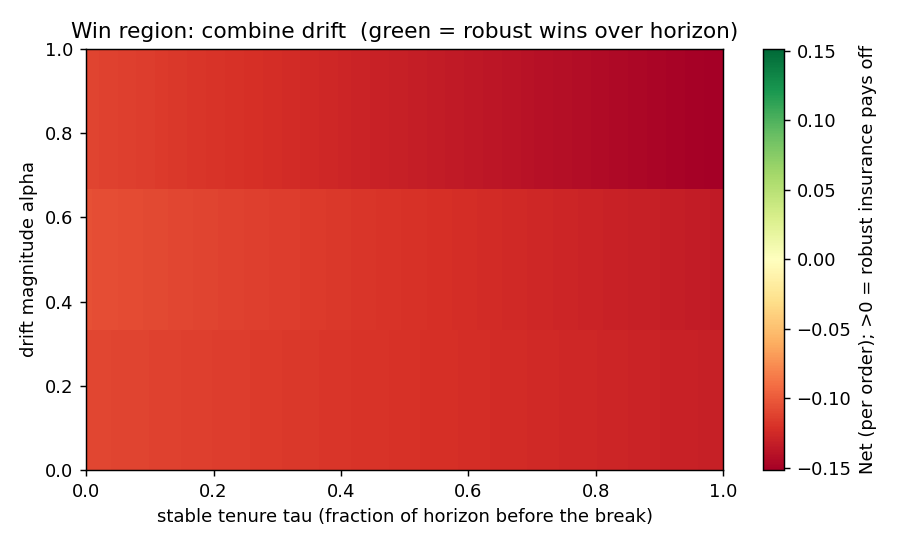
\includegraphics[width=0.48\linewidth]{../reports/figures/fig6_winregion_combine.png}\hfill
  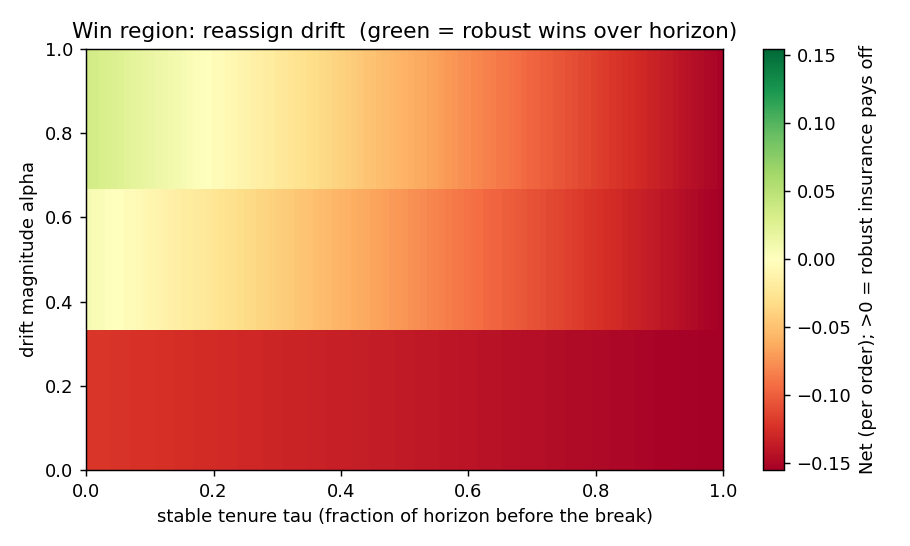
\includegraphics[width=0.48\linewidth]{../reports/figures/fig6_winregion_reassign.png}
  \caption{Sign of $\mathrm{Net}(\alpha,\tau)$ over the operating horizon, mode \emph{combine} (left) and mode \emph{reassign} (right). The robust layout pays off only where $\mathrm{Net}>0$. The region is empty: for any horizon with $\tau>0$ the price of the enlargement outweighs the out-of-sample saving.}
  \label{fig:rc-winregion}
\end{figure}

Two readings strengthen the negative. The data was constructed \emph{for} the method, with strong planted affinity and a future that grows exactly the within-community combinations the closures encode, and the method still lost; this is the opposite of a favorable-data critique. And the mechanism behind the loss is specific: the enlargement spreads the layout across more stations, broadening each group, and that spread is penalized precisely when future orders grow large, so the theoretically favorable \emph{combine} regime is empirically the worst one for the robust layout. The enlargement adds conservatism, a real price, without adding placement information the direct optimizer did not already have, because the direct min-visits solver performs the same transitive correlation clustering the cover encodes. The redundancy, not mere weakness, is why the result is break-even or worse across every lever.

% =====================================================================
\section{Why the outer-approximation cannot help here}\label{sec:rc-discussion}
% =====================================================================

The negative is consistent across the synthetic shift family, the clean $\kappa$-invariant Company~I instance, the controlled affinity drift even when rigged to favor the method, and the industrial Company~B instance once its capacity confound is removed. A single mechanism explains all of them. The explanation is specific to the CSLAP visit objective and we state it in that scope, not as a claim about robust optimization in general.

\paragraph{The placement objective is a well-estimated correlation-clustering objective.}
Minimizing total station visits is a correlation-clustering objective: products that co-occur in orders should share a station, and the optimal layout is the one that cuts the fewest co-occurring pairs across station boundaries. The direct nominal solver already optimizes this on the historical orders, and the optimum it finds depends on the data only through aggregate product co-occurrence counts. Those counts are a stable, low-variance statistic. They are estimated from a long order history, hundreds of thousands of orders on the industrial instances, so the sampling error in any single co-occurrence weight is small relative to the gaps between layouts. The nominal layout sits at a deterministic combinatorial optimum of a function whose inputs are sharply estimated. There is little estimation fragility for any robustification to protect.

\paragraph{The enlargement is a robust counterpart of the training objective with a trivial adversary.}
Proposition~\ref{prop:rc-identity} establishes that optimizing on the closures equals a static robust counterpart of the empirical objective. The robust reading is exact, but the inner maximization that defines it is trivial: by monotonicity of the visit function the adversary always plays the full closure, so the robust counterpart adds no genuine adversarial selection beyond mechanically enlarging every order. What enlargement does to the objective is make it coarser. The transformed objective is an upper bound on nominal visits whenever any closure strictly contains its order, and an upper bound is a biased surrogate for the quantity we actually pay. Optimizing a biased surrogate moves the selected layout away from the nominal optimum of the true objective. The further the closures grow, the coarser the surrogate and the larger this displacement.

\paragraph{A robust counterpart helps out of sample only against estimation fragility, which is absent here.}
A robust or distributionally robust counterpart improves generalization when the nominal solution is fragile, that is, when the objective is estimated with high variance and the nominal optimizer overfits sampling noise, so that worst-case hedging trades a little bias for a larger reduction in variance. The trade is favorable only when the variance term is large. Here it is not. The nominal CSLAP layout is a deterministic combinatorial optimum of co-occurrence counts that are themselves well estimated, so the variance the enlargement could remove is small, while the bias it introduces, through the coarser upper-bound surrogate, is real and grows with $\kappa$. The enlargement therefore buys bias without buying a commensurate reduction in variance. For this objective that is a strictly dominated trade: it can only move the out-of-sample cost in the wrong direction, which is exactly what every clean experiment shows. The price of robustness is the bias made visible on the training orders, and the negative out-of-sample gain is the same bias made visible on the test orders, with no offsetting variance reduction in between. The near-symmetry $\mathrm{PoR} \approx -G$ on Company~I is the signature of a pure bias term with no variance benefit.

\paragraph{The general claim, stated cautiously.}
For an objective of this kind, a deterministic correlation-clustering placement learned from a stable, well-sampled co-occurrence statistic, enlargement-based robustification is redundant with the direct optimizer. The direct min-visits solver already performs the transitive correlation clustering that the cover re-encodes, so the closures add conservatism without adding placement information. This is why the controlled \emph{combine} regime, built to be the textbook best case for the method, is empirically its worst case: growing future orders within the planted communities is the situation in which a layout spread across more stations is most heavily penalized, and the enlargement is exactly what spreads it. We do not claim the construction is useless for every uncertainty problem; we claim it cannot add out-of-sample value for this particular objective, because the object it protects against, estimation fragility of the nominal optimum, is not present.

\paragraph{The industrial subtlety: a capacity relaxation masquerading as robustness.}
The one place a positive gain appeared, Company~B in the first run, deserves the explicit mechanism, because it is instructive and because a careful test proved it was not the method. The first run loosened the workload constraint as a side effect of the recalibration formula~\eqref{eq:rc-Ts}, which rebuilt each station's time capacity $T_s$ from the inflated closure line counts. A binding workload constraint forces co-located products apart across stations: when a station's time capacity is tight, the placement model cannot put all the products of a tight co-occurrence cluster on one station and must split the cluster, which inflates visits on every order that touches it. Relaxing $T_s$ enlarges the feasible region and lets the optimizer cluster more freely, which lowers visits on the training orders and on the test orders alike. The decomposition in Section~\ref{sec:rc-berner-decomp-res} isolates this: arm~D, which loosens capacity with zero enlargement, delivers the entire gain and a negative price of robustness, proving the original cap was binding and that recalibration merely relaxed it. That relaxation is available to the nominal layout just as much as to the enlarged one, so it is not a property of the outer-approximation. The closures, isolated in arm~B, return a negative-to-break-even gain on their own, and they drag the loose-capacity arm down by about three percent. The apparent industrial robustness was a constraint relaxation, and once the constraint is held fixed at its real value the enlargement returns the same negative as everywhere else.

% =====================================================================
\section{Limitations}\label{sec:rc-limitations}
% =====================================================================

\paragraph{(a) Constrained versus true bottleneck.}
On the industrial instance the master saw a subsampled support set, so the stored bottleneck is $\Pi_{\text{constrained}}$ (34 at $\kappa=2$, 23 at $\kappa=3$), while the true bottleneck over the full stream of 142{,}241 distinct supports is $\Pi_{\text{true}}$ (369 at $\kappa=2$, 360 at $\kappa=3$). The worst-case bound of Proposition~\ref{prop:wc-bound} is therefore conditional on the full-stream bottleneck, and the subsampled construction does not certify global min-max optimality. The partition itself is valid on the full stream and Proposition~\ref{prop:rc-identity} is unaffected, since the identity depends only on monotonicity and on closures taken over all orders.

\paragraph{(b) Exact solver only for the cover, and only at reduced scale.}
The exact CPLEX backend (Section~\ref{sec:rc-iscf}) closes the first run's missing-exact-solver gap for the \emph{cover}: it reproduces the acceptance result as a certified-optimal $\Pi^\*=5$ and certifies $\Pi_{\text{true}}$ on the full support set of the controlled instance. Two parts remain inexact. The \emph{placement} runs on the Hexaly metaheuristic, not an exact MILP, so Proposition~\ref{prop:rc-identity}'s price-of-robustness inequality is observed empirically rather than at certified optimality, though $\mathrm{PoR}>0$ held in every fold regardless. And the exact integer master is tractable only up to a few hundred products at this support diversity: the full $4{,}328$-product Company~I cover did not certify within the session budget (an LP relaxation of $\Pi\approx73$ at $\kappa=2$ and a single master solve of several minutes on a $10^5$-column pool), so the controlled study uses the $480$-product sub-instance. The exact evaluation is therefore clean but at reduced scale.

\paragraph{(c) The recalibration side-channel, removed on both clean instances and decomposed on Company~B.}
On the first synthetic and Company~B runs the time-capacity recalibration \eqref{eq:rc-Ts} was applied on the enlarged arms, so $\mathrm{PoR}$ and $G$ there mixed enlargement with a capacity change. This is no longer a hedge but a measured effect. The clean Company~B rebuild and its two-by-two decomposition (Section~\ref{sec:rc-berner-decomp-res}) attribute the entire apparent gain to the capacity loosening: the capacity-only arm with zero enlargement delivers it in full and carries a negative price of robustness, so the original cap was binding. The Company~I evaluation removes the same confound by construction, since capacity is $\kappa$-invariant and the workload is driven by the real per-product pick-lines, so both arms share an identical capacity file and the measured $\mathrm{PoR}>0$ cannot be a recalibration artefact. The clean negatives of Sections~\ref{sec:rc-berner-decomp-res} and~\ref{sec:rc-iscf-res} are the readings that should be weighted most heavily.

\paragraph{(f) A single enlargement level on the clean instance.}
The exact study certifies only $\kappa=2$. The set-partition integer master does not reach optimality for $\kappa\ge3$ at this scale: a $\kappa=3$ run returned an incumbent bottleneck of $71$, larger than the certified $\kappa=2$ optimum of $49$, which is a solver failure since the optimal bottleneck is non-increasing in $\kappa$. The exact evaluation therefore yields a single point rather than a tradeoff curve, and does not test the predicted interior optimum on the clean instance. The placement objective there is also restricted to the most frequent multi-item supports for tractability, while evaluation uses all real orders.

\paragraph{(g) Scale of the exact Company~B decomposition.}
The clean Company~B decomposition (Section~\ref{sec:rc-berner-decomp-res}) restricts to the top-$2{,}000$ products so the exact CPLEX min-sum covers certify, rather than the full $21{,}316$-product universe. The escalation criterion for a full-scale rerun was a positive preprocess-only gain $G(B)$; since $G(B)$ is negative-to-break-even at every $\kappa$, the criterion is not met and the full-scale rerun is unnecessary at this scale. The decomposition is therefore exact on a reduced product set, and the conclusion it draws, that the apparent gain was capacity rather than the preprocess, holds on the structure it tested.

\paragraph{(d) Single-solver Company~B temporal cell.}
The original Company~B temporal hold-out of Section~\ref{sec:rc-berner-res} is a single cell on the greedy heuristic, because simulated annealing did not scale to the enlarged arms and the genetic algorithm degenerated to a seed-fixed layout at the 120-second budget. The decomposition of Section~\ref{sec:rc-berner-decomp-res} removes the interpretive weight that cell once carried, since the apparent gain is now explained, but the original temporal cut itself rests on one solver.

\paragraph{(e) Oracle probe scope.}
The relative-regret reading is a two-cell, single-seed probe at $\theta'=0.7$ with $\rho \in \{0, 1.0\}$, not the full grid. It indicates the direction of the mechanism and nothing stronger.

Throughout, the tradeoff figures are plotted against the realized enlargement $\bar c$ ($\kappa=2 \approx 1.75$, $\kappa=3 \approx 2.2$) rather than nominal $\kappa$, because the realized enlargement is what the layout actually sees and it differs from $\kappa$ whenever the cover saturates.

% =====================================================================
\section{Conclusion}\label{sec:rc-conclusion}
% =====================================================================

We recast CSLAP placement under demand shift as a covering-based instance transformation and proved it equals a data-driven static robust counterpart of the empirical objective (Proposition~\ref{prop:rc-identity}), solved exactly by the unchanged solvers because the inner maximization is trivial under monotonicity. That part is settled: the construction is sound, reusable, and has an exact robust-optimization reading rather than a heuristic analogy. The empirical question H1 adds on top of it, whether the conservative layout actually wins out of sample, is answered in the negative, and the negative is now confirmed on both real industrial instances under a $\kappa$-invariant capacity. On the clean, capacity-balanced Company~I instance with an exact column-generation cover, the price of robustness at $\kappa=2$ is positive and the out-of-sample gain is negative under both five-fold cross-validation and a temporal split, every fold agreeing and both confidence intervals excluding zero. On Company~B, the only place a positive gain ever appeared, a two-by-two decomposition that holds the workload capacity at its real value shows the apparent gain came entirely from a capacity relaxation: the outer-approximation alone returns a negative-to-break-even gain, while the capacity loosening alone, with zero enlargement, delivers the whole benefit and a negative price of robustness, the signature of a binding constraint relaxed rather than a layout made robust. The controlled affinity-drift stress-test closes the remaining objection that the real data simply does not drift: on data built to favor the method, with strong planted communities and a future that grows the combinations the closures encode, the win-region over the operating horizon is empty, because the out-of-sample saving is never significantly positive while the price is always paid.

These results share one mechanism, set out in Section~\ref{sec:rc-discussion}. The CSLAP visit objective is a correlation-clustering objective whose nominal optimum is a deterministic combinatorial solution of well-estimated co-occurrence counts, so there is no estimation fragility for a robust counterpart to protect. The enlargement adds conservatism, a bias visible as a positive price on training and a negative gain on test, without a compensating reduction in variance, which is a dominated trade for this objective. The direct min-visits solver already performs the transitive correlation clustering the cover re-encodes, so the closures are redundant with the direct optimizer rather than complementary to it. For a deterministic correlation-clustering placement learned from a stable, well-sampled co-occurrence statistic, enlargement-based robustification cannot add out-of-sample value, and the experiments are the empirical face of that statement. The honest finding is that H1 is \emph{not} supported: a covering enlargement that is provably a robust counterpart of the training objective does not translate into out-of-sample robustness for this problem.

The negative is specific and bounded, and three directions would test its edges. The exact study certifies a single enlargement level, $\kappa=2$, because the integer master does not reach optimality for larger $\kappa$ at this support diversity; a stronger integer formulation or a warm-started master would let the full $\mathrm{PoR}$--$G$ curve be traced and the predicted interior optimum be tested directly, rather than inferred from one point. Scaling the exact cover beyond a few hundred products would let the clean $\kappa$-invariant evaluation run on the largest industrial instance, where it is currently out of reach. And an enlargement object other than a min-max-$\Pi$ partition, for instance one weighted toward the products whose co-occurrence is most stable across time rather than most frequent, might enclose future orders more selectively than the uniform conservatism studied here; whether any such object turns the negative positive is open.

% =====================================================================
\section*{References}
% =====================================================================
% Verified references only (Stage-1 research report, 18 load-bearing items).
% No fabricated citations. Authors / venue / year / DOI as verified in-session.
\begin{thebibliography}{99}

\bibitem[Balas and Padberg(1976)]{balas1976}
Balas, E., Padberg, M.W., 1976. Set partitioning: a survey. SIAM Review 18(4), 710--760. DOI: 10.1137/1018115.

\bibitem[Karp(1972)]{karp1972}
Karp, R.M., 1972. Reducibility among combinatorial problems, in: Complexity of Computer Computations. Plenum Press, pp. 85--103. DOI: 10.1007/978-1-4684-2001-2\_9.

\bibitem[Ben-Tal and Nemirovski(1999)]{bental1999}
Ben-Tal, A., Nemirovski, A., 1999. Robust solutions of uncertain linear programs. Operations Research Letters 25(1), 1--13. DOI: 10.1016/S0167-6377(99)00016-4.

\bibitem[Bertsimas and Sim(2004)]{bertsimas2004}
Bertsimas, D., Sim, M., 2004. The price of robustness. Operations Research 52(1), 35--53. DOI: 10.1287/opre.1030.0065.

\bibitem[Bertsimas et al.(2011)]{bbc2011}
Bertsimas, D., Brown, D.B., Caramanis, C., 2011. Theory and applications of robust optimization. SIAM Review 53(3), 464--501. DOI: 10.1137/080734510.

\bibitem[Delage and Ye(2010)]{delage2010}
Delage, E., Ye, Y., 2010. Distributionally robust optimization under moment uncertainty with application to data-driven problems. Operations Research 58(3), 595--612. DOI: 10.1287/opre.1090.0741.

\bibitem[Mohajerin Esfahani and Kuhn(2018)]{esfahani2018}
Mohajerin Esfahani, P., Kuhn, D., 2018. Data-driven distributionally robust optimization using the Wasserstein metric. Mathematical Programming 171(1--2), 115--166. DOI: 10.1007/s10107-017-1141-8.

\bibitem[Bertsimas et al.(2018)]{bgk2018}
Bertsimas, D., Gupta, V., Kallus, N., 2018. Data-driven robust optimization. Mathematical Programming 167(2), 235--292. DOI: 10.1007/s10107-017-1125-8.

\bibitem[Birge and Louveaux(2011)]{birge2011}
Birge, J.R., Louveaux, F., 2011. Introduction to Stochastic Programming, 2nd ed. Springer. DOI: 10.1007/978-1-4614-0237-4.

\bibitem[Kleywegt et al.(2002)]{kleywegt2002}
Kleywegt, A.J., Shapiro, A., Homem-de-Mello, T., 2002. The sample average approximation method for stochastic discrete optimization. SIAM Journal on Optimization 12(2), 479--502. DOI: 10.1137/S1052623499363220.

\bibitem[Heitsch and R\"omisch(2003)]{heitsch2003}
Heitsch, H., R\"omisch, W., 2003. Scenario reduction algorithms in stochastic programming. Computational Optimization and Applications 24(2--3), 187--206. DOI: 10.1023/A:1021805924152.

\bibitem[Rockafellar and Wets(1991)]{rockafellar1991}
Rockafellar, R.T., Wets, R.J.-B., 1991. Scenarios and policy aggregation in optimization under uncertainty. Mathematics of Operations Research 16(1), 119--147. DOI: 10.1287/moor.16.1.119.

\bibitem[de Koster et al.(2007)]{dekoster2007}
de Koster, R., Le-Duc, T., Roodbergen, K.J., 2007. Design and control of warehouse order picking: a literature review. European Journal of Operational Research 182(2), 481--501. DOI: 10.1016/j.ejor.2006.07.009.

\bibitem[Reyes et al.(2019)]{reyes2019}
Reyes, J.J.R., Solano-Charris, E.L., Montoya-Torres, J.R., 2019. The storage location assignment problem: a literature review. International Journal of Industrial Engineering Computations 10(2), 199--224. DOI: 10.5267/j.ijiec.2018.8.001.

\bibitem[Mantel et al.(2007)]{mantel2007}
Mantel, R.J., Schuur, P.C., Heragu, S.S., 2007. Order oriented slotting: a new assignment strategy for warehouses. European Journal of Industrial Engineering 1(3), 301--316. DOI: 10.1504/EJIE.2007.014689.

\bibitem[Xiao and Zheng(2012)]{xiao2012}
Xiao, J., Zheng, L., 2012. Correlated storage assignment to minimize zone visits for BOM picking. International Journal of Advanced Manufacturing Technology 61(5--8), 797--807. DOI: 10.1007/s00170-011-3740-5.

\bibitem[Zhang et al.(2019)]{zhang2019}
Zhang, R.-Q., Wang, M., Pan, X., 2019. New model of the storage location assignment problem considering demand correlation pattern. Computers \& Industrial Engineering 129, 210--219. DOI: 10.1016/j.cie.2019.01.027.

\bibitem[Gademann and van de Velde(2005)]{gademann2005}
Gademann, N., van de Velde, S., 2005. Order batching to minimize total travel time in a parallel-aisle warehouse. IIE Transactions 37(1), 63--75. DOI: 10.1080/07408170590516917.

\bibitem[Kofler et al.(2014)]{kofler2014}
Kofler, M., Beham, A., Wagner, S., Affenzeller, M., 2014. Affinity based slotting in warehouses with dynamic order patterns, in: Advanced Methods and Applications in Computational Intelligence. Topics in Intelligent Engineering and Informatics, vol. 6, Springer, pp. 123--143. DOI: 10.1007/978-3-319-01436-4\_7.

\end{thebibliography}

\end{document}
